\chapter{Preliminary Concepts and Formulations}\label{chp:preliminary-concepts}

In this chapter, we introduce the fundamental concepts necessary for
understanding this thesis. The basic notation and definitions are presented in
Section~\ref{sec:not-e-def}. In this work, we employ basic concepts from
Combinatorial Optimization, which are assumed to be known. If the reader deems a
review necessary, we recommend the textbook by Nemhauser and
Wolsey~\cite{Nemhauser}, which covers this topic with a focus on \gls{ilp}, one
of the main tools used in this work. Basic concepts related to graph theory are
also assumed to be known. Should the
reader require a refresher, the material can be found in standard textbooks on
the subject, such as Diestel~\cite{diestel:2005}. 

% TODO: add references to the sections
The mathematical models are presented in Sections~\ref{sec:dmfm-pma}
and~\ref{sec:ab-pma}. Section~\ref{sec:rel-lagrangiana} provides a description
of the functioning and application of Lagrangian relaxation, one of the main
approaches employed in this work. Finally, in Sections~\ref{sec:metaheuristic}
and~\ref{subsec:brkga}, we present a general discussion on metaheuristics.


\section{Notations and Definitions} \label{sec:not-e-def}

Once a spraying vehicle begins to service a city block, it must sequentially
cover all surrounding edges in a clockwise direction. The
traversal ensures that the insecticide fog forms a continuous barrier,
preventing mosquitoes from escaping. 
The clockwise direction is due to real operational factors, 
as the nebulizer equipment points to the right side of the
vehicle. 
Figure~\ref{fig:instance_digraph_fumace_car} shows an example of a map,
with four blocks to service, and Figure~\ref{fig:route_fumace_car} presents a
spraying route for these blocks where the nebulizer is activated in the black
dots and follows the direction of the arrow, starts by serving Block 2, goes to
Blocks 1, 3 and 4, respectively.

\begin{figure}[h!]
	\begin{minipage}[c]{.49\textwidth}
		\centering
		\subfloat[A CBRP instance
			digraph.]{\label{fig:instance_digraph_fumace_car}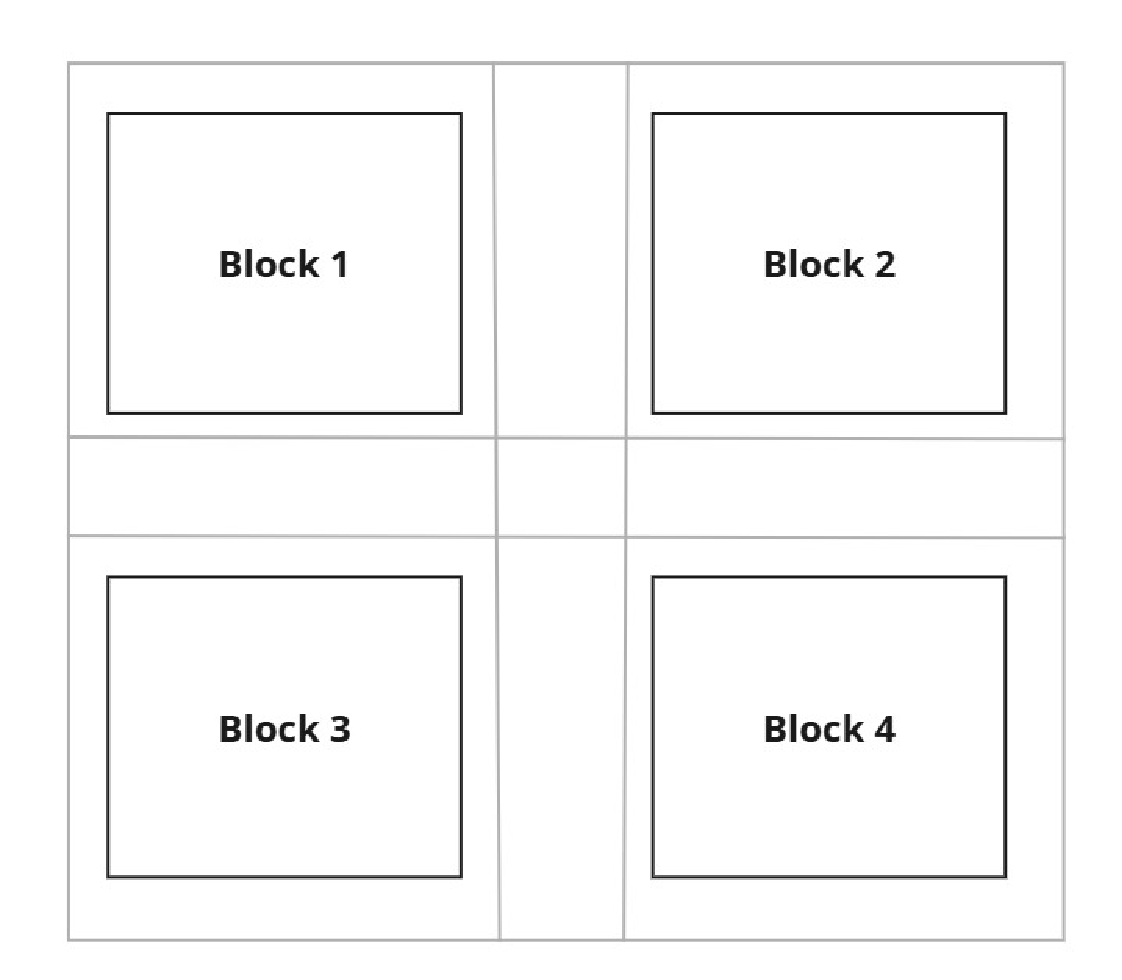
\includegraphics[width=5cm,
				height=5cm]{images/cbrp-instance.pdf}} \end{minipage}%
	\begin{minipage}[c]{.49\textwidth}
		\centering
		\subfloat[A spraying vehicle route covering four city
			blocks.]{\label{fig:route_fumace_car}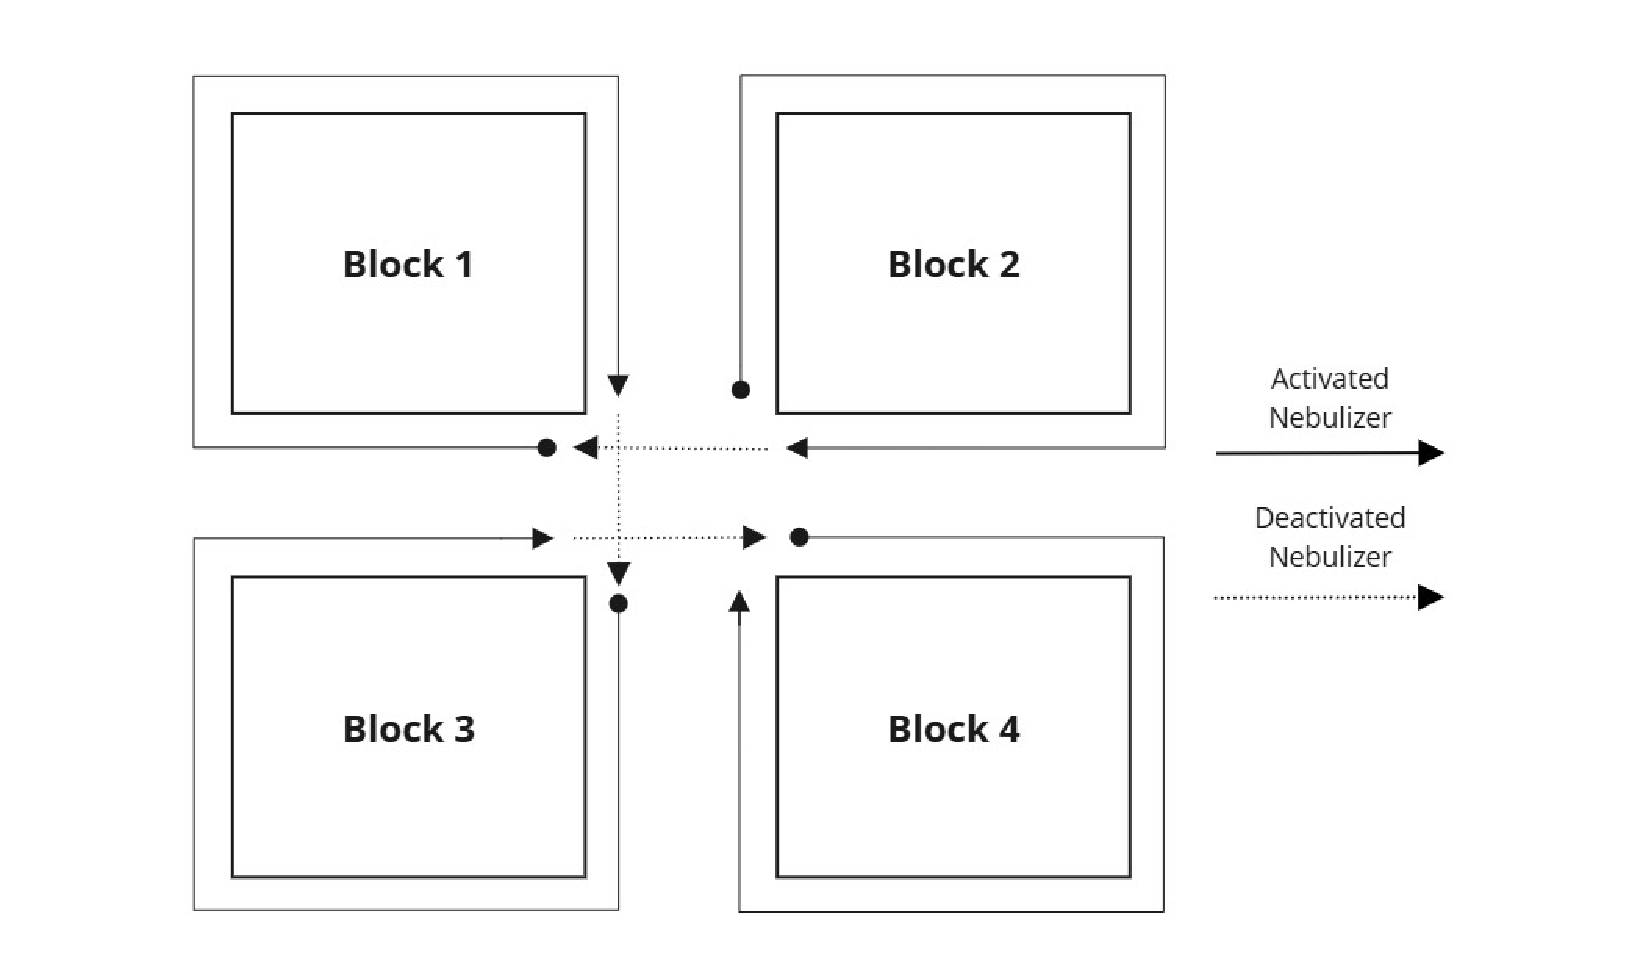
\includegraphics[width=8cm,
				height=5cm]{images/nebulizer-activated.pdf}}
	\end{minipage}
	\caption{\label{fig:route-ex} CBRP example.}
\end{figure}


Let $G = (V, A, B)$ be a weighted and directed graph, where $V = \{1, \dots, n\}$
is the set of vertices, $A = \{(i, j) : i, j \in V, i \neq j\}$
is the set of $m$ arcs, and $B = \{b : b \subseteq V\}$ is the set of blocks.
In each arc, the first vertex is the source and also the
predecessor of the second vertex in the ordered pair, which is known as the
destination. Each block $b$ has an associated set of arcs $B(i, j) \subseteq A$ that
can be serviced by a vehicle. 

We now present a formal definition of the \gls{cbrp}. Let a Plannar Graph,
extracted from a real citymap, be represented as a weighted directed graph
$G$. Each node in $V$ represents the intersection of at least two
streets and has a list of blocks $b \subseteq B$ that are associated with it.
Each arc $(i, j) \in A$ has a deadheading time $t_{i, j} > 0$, a service time
$t^{'}_{i, j} > 0$ such that $t_{i, j} \leqslant t^{'}_{i, j}$ and the block
$b \in B$ that is associated with it. The input to the \gls{cbrp} is defined as:

\begin{itemize}
	\item $G = (V, A, B)$ is a weighted directed planar graph with the blocks associated with it;
	\item $p_b : B \rightarrow \mathbb{N}$ is a function that returns the profit
	      for each block $b \in B$;
	\item $t_{i, j} : A \rightarrow \mathbb{N}$ is a function that returns the
	      deadheading time for each arc $(i, j) \in A$;
	\item $t^{'}_{i, j} : A \rightarrow \mathbb{N}$ is a function that returns
	      the service time for each arc $(i, j) \in A$;
	\item $T$ is the time limit for the vehicle to travel and service the blocks;
	\item $V(b)$ is the set of nodes that are associated with the block $b \in B$;
	\item $B(i)$ is the set of blocks that are associated with the node $i \in V$;
	\item $B(i, j)$ is the set of blocks that are associated with the arc $(i, j) \in A$;
	\item $\delta^{+}_{i}$ is the set of arcs with destination $i$;
	\item $\delta^{-}_{i}$ is the set of arcs with source $i$;
\end{itemize}

The \gls{cbrp} is introduced as a general framework for addressing the routing of
spraying vehicles and other city block servicing problems. 
The objective of the \gls{cbrp} is to determine an optimal traversal that 
services a subset of blocks within a network, maximizing the total 
collected benefit from each serviced block. 
A vehicle traverses the graph $G$ following a route that can serve a
subset of blocks within a given time limit $T$. This work considers two types of 
solution routes, depending on whether the vertices can be
visited more than once: \textit{Walk-based route}, in which any vertex (or arc)
can be visited multiple times and \textit{Path-based route}, in which no vertex
appears more than once. 
An optimal route (walk or path) is one that maximizes
the total prize collected from the serviced blocks while respecting the vehicle
time limit $T$.

To facilitate modeling, we augment the graph $G$ by introducing a dummy depot
$0$, from which the route originates, and a set of arcs $\{(0, i), (i, 0) :
	\forall i \in V\}$ with times $t_{i,0} = t_{0,i} = 0$, $\forall i \in V$. 
Thus, we define the modified graph as $G' = (V' = V \cup \{0\}, A' = A \cup \{(0,
	i), (i, 0) : \forall i \in V\})$.

We now present key properties of the \gls{cbrp}. First, due to the operational
restrictions, once a block $b$ starts being serviced at a given node $i$, it
must be fully encircled before the vehicle moves to another block. This leads
to the following property:

\begin{property}
	\label{claim:core_insight}
	A block can be serviced if at least one of its nodes is visited.
\end{property}

From Property~\ref{claim:core_insight}, 
when formulating the problem, it is not
necessary to explicitly require the vehicle to completely traverse a block's
perimeter in order to count it as serviced. Instead, servicing can be achieved
by visiting at least one node within the block and accounting for the
corresponding service time. This property is valid due to the definition of the blocks $B$ and
the fact that the vehicle must service all blocks in a clockwise direction.

Figure~\ref{fig:servicing_block_no_surrounding_strategy} illustrates an example of
this strategy, where servicing is achieved without requiring a full traversal of
the block's perimeter.

\begin{figure}[!ht]
	\begin{minipage}[c]{.32\textwidth}
		\begin{tikzpicture}[
				> = stealth, % arrow head style
				shorten > = 0.8pt, % don't touch arrow head to node
				auto,
				node distance = 1.4cm, % distance between nodes
				semithick % line style
			]
			
			\tikzstyle{every state}=[
			draw = black,
			thick,
			fill = white,
			minimum size = 9mm
			]
			
			\node[state] (a) at (0,0) {$1$};
			\node[state, right of = a] (b) {$2$};
			\node[state, above of = a] (c) {$3$};
			\node[state, above of = b] (d) {$4$};
			
			\node[state, right of = b, xshift=0.3cm] (e) {$5$};
			\node[state, right of = d, xshift=0.3cm] (f) {$6$};
			\node[state, right of = e] (g) {$7$};
			\node[state, right of = f] (h) {$8$};
			
			\node[state, below of = b, yshift=-0.5cm] (i) {$9$};
			\node[state, below of = e, yshift=-0.5cm] (j) {$10$};
			\node[state, below of = i, left of = j, xshift=0.5cm] (k) {$11$};
			
			\path[->, draw = gray, opacity = 0.2] (a) edge node {} (c); 
			\path[->, draw = gray, opacity = 0.2] (c) edge node {} (d); 
			\path[->, draw = gray, opacity = 0.2] (d) edge node {} (b);
			\path[->, draw = gray, opacity = 0.2] (b) edge node {} (a);
			
			\path[->, draw = gray, opacity = 0.2] (e) edge node {} (f);
			\path[->, draw = gray, opacity = 0.2] (f) edge node {} (h);
			\path[->, draw = gray, opacity = 0.2] (h) edge node {} (g);
			\path[->, draw = gray, opacity = 0.2] (g) edge node {} (e);
			
			\path[->, draw = gray, opacity = 0.2] (i) edge node {} (j);
			\path[->, draw = gray, opacity = 0.2] (j) edge node {} (k);
			\path[->, draw = gray, opacity = 0.2] (k) edge node {} (i);
			
			\path[->, draw = gray, opacity = 0.2, dashed] (j) edge node {} (b);
			\path[->, draw = gray, opacity = 0.2, dashed] (b) edge node {} (e);
		\end{tikzpicture}
		\subcaption{Instance Example.}
	\end{minipage}
	\hfill
	\begin{minipage}[c]{.32\textwidth}
		\begin{tikzpicture}[
				> = stealth, % arrow head style
				shorten > = 0.8pt, % don't touch arrow head to node
				auto,
				node distance = 1.4cm, % distance between nodes
				semithick % line style
			]
			
			\tikzstyle{every state}=[
			draw = black,
			thick,
			fill = white,
			minimum size = 9mm
			]
			
			\node[state] (a) at (0,0) {$1$};
			\node[state, right of = a] (b) {$2$};
			\node[state, above of = a] (c) {$3$};
			\node[state, above of = b] (d) {$4$};
			
			\node[state, right of = b, xshift=0.3cm] (e) {$5$};
			\node[state, right of = d, xshift=0.3cm] (f) {$6$};
			\node[state, right of = e] (g) {$7$};
			\node[state, right of = f] (h) {$8$};
			
			\node[state, below of = b, yshift=-0.5cm] (i) {$9$};
			\node[state, below of = e, yshift=-0.5cm] (j) {$10$};
			\node[state, below of = i, left of = j, xshift=0.5cm] (k) {$11$};
			
			\path[->, draw = gray, opacity = 1.0] (a) edge node {} (c); 
			\path[->, draw = gray, opacity = 1.0] (c) edge node {} (d); 
			\path[->, draw = gray, opacity = 1.0] (d) edge node {} (b);
			\path[->, draw = gray, opacity = 1.0] (b) edge node {} (a);
			
			\path[->, draw = gray, opacity = 1.0] (e) edge node {} (f);
			\path[->, draw = gray, opacity = 1.0] (f) edge node {} (h);
			\path[->, draw = gray, opacity = 1.0] (h) edge node {} (g);
			\path[->, draw = gray, opacity = 1.0] (g) edge node {} (e);
			
			\path[->, draw = gray, opacity = 1.0] (i) edge node {} (j);
			\path[->, draw = gray, opacity = 1.0] (j) edge node {} (k);
			\path[->, draw = gray, opacity = 1.0] (k) edge node {} (i);
			
			\path[->, draw = gray, opacity = 1.0, dashed] (j) edge node {} (b);
			\path[->, draw = gray, opacity = 1.0, dashed] (b) edge node {} (e);
		\end{tikzpicture}
		\subcaption{Explicity Block Servicing.}
	\end{minipage}\\
	\centering
	\begin{minipage}[c]{.32\textwidth}
		\begin{tikzpicture}[
				> = stealth, % arrow head style
				shorten > = 0.8pt, % don't touch arrow head to node
				auto,
				node distance = 1.4cm, % distance between nodes
				semithick % line style
			]
			
			\tikzstyle{every state}=[
			draw = black,
			thick,
			fill = white,
			minimum size = 9mm
			]
			
			\node[state] (a) at (0,0) {$1$};
			\node[state, right of = a] (b) {$2$};
			\node[state, above of = a] (c) {$3$};
			\node[state, above of = b] (d) {$4$};
			
			\node[state, right of = b, xshift=0.3cm] (e) {$5$};
			\node[state, right of = d, xshift=0.3cm] (f) {$6$};
			\node[state, right of = e] (g) {$7$};
			\node[state, right of = f] (h) {$8$};
			
			\node[state, below of = b, yshift=-0.5cm] (i) {$9$};
			\node[state, below of = e, yshift=-0.5cm] (j) {$10$};
			\node[state, below of = i, left of = j, xshift=0.5cm] (k) {$11$};
			
			\path[->, draw = gray, opacity = 0.2] (a) edge node {} (c); 
			\path[->, draw = gray, opacity = 0.2] (c) edge node {} (d); 
			\path[->, draw = gray, opacity = 0.2] (d) edge node {} (b);
			\path[->, draw = gray, opacity = 0.2] (b) edge node {} (a);
			
			\path[->, draw = gray, opacity = 0.2] (e) edge node {} (f);
			\path[->, draw = gray, opacity = 0.2] (f) edge node {} (h);
			\path[->, draw = gray, opacity = 0.2] (h) edge node {} (g);
			\path[->, draw = gray, opacity = 0.2] (g) edge node {} (e);
			
			\path[->, draw = gray, opacity = 0.2] (i) edge node {} (j);
			\path[->, draw = gray, opacity = 0.2] (j) edge node {} (k);
			\path[->, draw = gray, opacity = 0.2] (k) edge node {} (i);
			
			\path[->, draw = gray, opacity = 1.0, dashed] (j) edge node {} (b);
			\path[->, draw = gray, opacity = 1.0, dashed] (b) edge node {} (e);
		\end{tikzpicture}
		\subcaption{Implicit Block Servicing.}
	\end{minipage}
	\caption{\label{fig:servicing_block_no_surrounding_strategy} Strategies for servicing blocks.}
\end{figure}

\section{Deterministic Models} \label{sec:cbrp-deterministic-models}

Given as instance for the \gls{cbrp}, consider a path-based solution on the
original planar graph, in which no arc or vertex is visited more than once. The
following binary decision variables are introduced for the model:

\begin{itemize}
	\item $x_{ij} \in \{0, 1\}$ is a binary variable that indicates whether the arc $(i, j) \in A'$ is included in the route ($x_{ij} = 1$) or not ($x_{ij} = 0$);
	\item $y_{ib} \in \{0, 1\}$ is a binary variable that indicates whether node $i \in V$ is selected as the starting point for serving block $b \in B(i)$ ($y_{ib} = 1$) or not ($y_{ib} = 0$).
\end{itemize}

The Path-CBRP formulation is defined as follows:

\begin{align}
	\text{(Path-CBRP) }          & \max \sum_{i \in V} \sum_{b \in B} p_b y_{ib}                                             & \label{eq:of}                                                  \\
	\nonumber \text{subject to:} &                                                                                           &                                                                \\
	                             & \sum_{i \in V} x_{0,i} = \sum_{j \in V} x_{j,0} = 1                                       & \label{eq:s-t-all}                                             \\
	%
	                             & \sum_{i \in V} x_{i,j} - \sum_{k \in V} x_{j,k} = 0                                       & \ \forall j \in V \label{eq:flow-conservation}                 \\
	%
	                             & \sum_{i \in V(b)} y_{ib} \leq 1                                                           & \ \forall b \in B \label{eq:max-attend}                        \\
	%
	                             & \sum_{j \in \delta^{-}(i)} x_{i,j} \geq y_{ib}                                            & \ \forall b \in B, i \in V(b) \label{eq:in-path}               \\
	%
	                             & \sum_{(i, j) \in A} x_{i,j}t_{i,j} + \sum_{i \in V} \sum_{b \in B} y_{ib}t^{'}_{b} \leq T & \label{eq:max-time}                                            \\
	                             & \sum_{(i, j) \in A(S)} x_{i,j} \leq |V(S)| - 1                                            & \ \forall S \subseteq V \label{eq:circuit-subtour-elimination} \\	
	                             & x \in \mathbb{B}^{|A'|}                                                                   & \label{eq:dom-x}                                               \\
	                             & y \in \mathbb{B}^{|V'| * |B|}.                                                            & \label{eq:dom-y}
\end{align}


The Path-CBRP formulation generates a closed path that starts and ends at the
depot. The objective function~\eqref{eq:of} maximizes the total prize collected
from each serviced block.
Constraints~\eqref{eq:s-t-all}-\eqref{eq:flow-conservation} enforce the start
and end of the route at the depot, and the flow conservation at each node, i.e.
the number of arcs entering a node equals to the number of arcs leaving it.
Constraints~\eqref{eq:max-attend} and~\eqref{eq:in-path} ensure that exactly one
node is selected as the starting point for servicing a block.
Constraints~\eqref{eq:max-time} impose a time limit, accounting for differences
in time spent while servicing and traveling.
Constraints~\eqref{eq:circuit-subtour-elimination} prevent the
formation of subcycles. Finally, constraints~\eqref{eq:dom-x} and~\eqref{eq:dom-y}
define the domain of the decision variables.

Since the subcycle elimination constraints are exponentially large in relation
to the input size, there are two most common approaches to solve Path-CBRP:
the first is to apply the subcycle elimination procedure to integer solutions
obtained during the solver branch and bound. The second is to replace the
constraint by a more compact set of constraints based on the \gls{mtz}
formulation.

% TODO: move to a future subsection with more details
% The implementation of the subtour elimination constraint leads to a separation
% heuristic using max-flow/min-cut that is applied in fractional branch and bound
% solutions. Arc capacities are derived from their relaxed LP solution values. The
% sum of arcs in the identified min-cut must carry at least the flow indicated by
% \( y_{ib} \) variables on either side of the cut. The preflow min-cut algorithm
% from the Lemon Library~\citep{lemon:2011} is used.

To implement the \gls{mtz} approach, we introduce the following additional
variable: 

\begin{itemize}
	\item $w_{a} \in \mathbb{R}$ is a real-valued variable representing the accumulated
	      time along the arc $(i, j) \in A'$.
\end{itemize}

Using this variable, it is possible to replace the constraints~\eqref{eq:max-time}-\eqref{eq:circuit-subtour-elimination}
by the following set of constraints:

\begin{align}
	 & w_{j,k} \geq w_{i,j} + x_{i,j}t_{i,j} - (2 - x_{j,k} - x_{i,j})T & \forall (i, j) \in A, (j, k) \in A, j \in V \label{eq:max-time-compact-leq}                               \\
	 & w_{i,0} \leq T                                                   & \forall i \in V.                                                            & \label{eq:max-time-compact}
\end{align}

Constraints~\eqref{eq:max-time-compact-leq} compute the accumulated time at each
arc, while constraints~\eqref{eq:max-time-compact} enforce an upper bound on the
\gls{mtz} variable. This reformulated model maintains an equivalent set of integer
feasible solutions to Path-CBRP while significantly reducing the number of
constraints, which now grows polynomially with respect to the input size.
However, the fractional feasible space may widen, since the number of cuts
reduced from exponential to polynomial. This formulation is referred to as
Path-CBRP-MTZ.

\section{Walk Solution} \label{sec:cbrp-walk-solution}

% Change to maximization problem

\section{Lagrangean Relaxation} \label{sec:cbrp-lagrangean-relaxation}

\gls{lr} is a well-known decomposition method used to solve combinatorial
optimization problems. The main idea of \gls{lr} is to remove complicated
constraints from the mathematical model and transfer them to the objective
function by assigning them weights (known as Lagrange multipliers), which
penalize their violation in any solution. It can be shown that the cost of an
optimal solution to the \gls{lr} always provides a dual bound for the optimal
value of the original problem. A primal bound can be obtained by checking the
feasibility of a solution returned by the relaxed model and computing the value
of the original objective function for that solution. An important step in
\gls{lr} is determining the values of the Lagrange multipliers that yield the
best dual bound. For this purpose, the subgradient method can be employed, which
is an iterative procedure in which the multipliers are updated until they
converge to their optimal values. For a minimization problem, this method can be
interpreted as the maximization of the lower bound obtained from the relaxed
model based on appropriate choices of multipliers~\cite{Beasley:1993}.

\gls{lr} is particularly convenient for problems that, apart from a subset of
complicating constraints, can be efficiently solved. For instance, consider the
following \gls{ilp} model:

\begin{align*}
	\text{(IP) } &              &  & z = \min cx           &  &  &  &  &  &  &  &   \\
	             & \text{s.t. } &  & Ax \geq b,            &  &  &  &  &  &  &  &   \\
	             &              &  & Dx \geq d,            &  &  &  &  &  &  &  &   \\
	             &              &  & x \in \mathbb{Z}^n_+. &  &  &  &  &  &  &  & 
\end{align*}

Assuming $Dx \geq d$ is the set of complicating constraints, removing it yields
$z' = \min \{cx : x \in X\}$, where $X = \{x \in \mathbb{Z}^n_+ : Ax \geq b\}$,
which is an easier problem and referred to as the relaxed problem. Two facts can
be observed. First, $z'$ is a lower (dual) bound on $z$, since the feasible
region of $x$ is larger, so the optimal value of $z'$ is less than or equal to
that of $z$. Second, the optimal solution in $X$ may not satisfy the constraints
in $Dx \geq d$. Based on these observations, the idea is to move the
complicating constraints into the objective function, penalizing their violation
using a vector $u \in \mathbb{R}^{m}_+$. This results in the Lagrangian
relaxation problem (\gls{lpp}), which can be written as:

\begin{align*}
	\text{LR($u$) } &              &  & z(u) = \min cx + u(d - Dx) &  &  &  &  &  &  &   \\
	                & \text{s.t. } &  & x \in X,                   &  &  &  &  &  &  &   \\
	                &              &  & u \in \mathbb{R}^m_+.      &  &  &  &  &  &  & 
\end{align*}

The following proposition establishes the relationship between $z(u)$ and $z$.

\begin{proposition}
	Let $z(u) = \min \{cx + u (d - Dx) : x \in X\}$. Then, $z(u) \leq z$ for all $u \geq 0$.
\end{proposition}

The penalty $u_i$ associated with constraint $D_ix \geq d_i$ is called the
Lagrange multiplier for that constraint. We now define the following problem:
determine the set of multipliers that provide the best (i.e., greatest) dual
bound $z(u)$. To find these values, we must solve the Lagrangian dual problem
(\gls{ldp}), described as:

\begin{align*}
	\text{LD } &  &  & w = \max \{z(u) : u \geq 0\}. &  &  &  &  & 
\end{align*}

The Lagrangian dual can be solved using the subgradient optimization method,
which is based on the following result.

\begin{proposition} \label{proposition:convex}
	A function $g : \mathbb{R}^n \rightarrow \mathbb{R}$ is concave if and only if, for every $\bar{x} \in \mathbb{R}^n$, there exists $s \in \mathbb{R}^n$ such that $g(\bar{x}) + s(x - \bar{x}) \geq g(x)$ for all $x \in \mathbb{R}^n$.
\end{proposition}

Thus, at point $\bar{x}$, it is necessary to choose a direction in which to move
to increase $g(x)$. From Proposition~\ref{proposition:convex}, we know that if
$g(x) > g(\bar{x})$, then $s(x - \bar{x}) > 0$. That is, moving an appropriate
amount in the direction of $s$ from $\bar{x}$ will increase the value of $g$.
Therefore, we must find a vector $s$ that satisfies
Proposition~\ref{proposition:convex}. When $g$ is differentiable at $\bar{x}$,
we can take $s = \nabla g(\bar{x})$, i.e., the gradient of $g$ at $\bar{x}$.
However, when $g$ is not differentiable, Proposition~\ref{proposition:convex}
still guarantees the existence of a vector $s$ such that $s(x^* - \bar{x}) > 0$
for an optimal point $x^*$. This means it is possible to move from $\bar{x}$ a
small step in the direction of $s$ to get closer to an optimal point, even if
$g$ does not increase. Before finding such a vector $s$, we define the notions
of subgradient and subdifferential.

\begin{definition}\label{definition:subgradient}
	Let $g : \mathbb{R}^n \rightarrow \mathbb{R}$ be a concave function. A vector $s$ is a subgradient of $g$ at $\bar{x}$ if and only if $s(x - \bar{x}) \geq g(x) - g(\bar{x})$ for all $x \in \mathbb{R}^n$. The subdifferential $(\delta g(\bar{x}))$ of $g$ at $\bar{x}$ is the set of all subgradients at that point.
\end{definition}

An immediate consequence of the above is the following:

\begin{proposition}\label{proposition:optimal}
	If $g$ is concave and $0 \in \delta g(x^*)$, then $g(x^*) = \max\{g(x) : x \in \mathbb{R}^n\}$, that is, $x^*$ is an optimal solution.
\end{proposition}

Therefore, in theory, to maximize a concave function $g$, it is sufficient to
start from any point and iteratively take small steps in the direction of a
subgradient at that point until $0$ belongs to the subdifferential of the
current point—that is, the current point is optimal. The results below allow us
to apply this theory to the Lagrangian relaxation technique for \gls{ilp}.

\begin{proposition} \label{proposition-zu-convex}
	$z(u) = \min \{cx + u (d - Dx)\}$ is concave.
\end{proposition}

The next result shows how to compute a subgradient of $z(u) = \min \{cx + u (d -
	Dx) : x \in X\}$ at point $u$.

\begin{proposition}
	Let $\bar{x} \in X$ such that $z(u) = c \bar{x} + u(d - D\bar{x})$. Then, $(d - D\bar{x})$ is a subgradient of $z(u)$ at $u$.
\end{proposition}

Based on the previous definitions and results, we can now present a procedure to
minimize a concave function for which a subgradient is known at all points in
its domain. For this purpose, a high-level pseudocode of the subgradient method
is presented in Algorithm~\ref{code:subgradient}.

\begin{algorithm}[!ht]
	\caption{\label{code:subgradient} Subgradient Method (Minimization Problem)}
	\Input{threshold, maxIter, updatePi}
	\Output{$z_{LB}$, $z_{UB}$}
	$m \leftarrow \rho \leftarrow 0$\;
	$z_{LB} \leftarrow 0$\;
	$z_{UB} \leftarrow$ cost of a feasible solution\;
	$\alpha^{0} \leftarrow \theta^{0} \leftarrow 0$\; $\pi^{0} \leftarrow 2$\;
	
	\While{$(\frac{z_{UB} - z_{LB}}{Z_{UB}}) \leq \ threshold$  or $m \ < \ maxIter$}{
		$x \leftarrow$ solution of $LR(\alpha^{m})$\;
		$z^{m} \leftarrow$ cost of the objective function of $x$ \;
		\If{$z^{m} > z_{LB}$}{
			$z_{LB} \leftarrow z^{m}$\;
		}
		$z_f^m \leftarrow$ original objective function value of solution $x$\;
		\uIf{$x$ is feasible and $z_f^m < z_{UB}$}{
			$z_{UB} \leftarrow z_f^m$\;
			$\rho \leftarrow 0$\;
		} \Else {
			$\rho \leftarrow \rho + 1$\;
		}
		
		\If{$\rho \ = \ updatePi$}{
			$\pi \leftarrow \pi/2$\;
			$\rho \leftarrow 0$\;
		}
		
		$\theta^{m} \leftarrow$ subgradient($x$)\;
		$n^{m} \leftarrow $ norm($\theta^{m}$)\;
		$s^{m} \leftarrow \pi^{m} \frac{(z_{UB} - z^{m})}{(n^{m})^{2}}$\;
		
		$\alpha^{m+1} \leftarrow \max(0, \alpha^{m} + s^{m}\theta^{m})$\;
		
		$m \leftarrow m + 1$\;
	}
\end{algorithm}

The algorithm takes three input parameters: `threshold`, `maxIter`, and
`updatePi`. The first two are stopping criteria. The `threshold` indicates the
maximum gap value for the solution to be considered optimal, terminating the
execution. The `maxIter` limits the maximum number of iterations of the
subgradient method. The third parameter, `updatePi`, is a counter for updating
the value of $\pi$, i.e., when `updatePi` consecutive iterations occur without
improvement in the dual bound. Lines (1)–(5) represent the initialization of
variables: $m$ is the main loop counter, and $\rho$ counts consecutive
iterations without improvement in $z_{UB}$. The variables $z_{LB}$ and $z_{UB}$
are the lower and upper bounds, respectively. The symbol $\alpha$ represents the
vector of Lagrange multipliers, and $\theta$ is the subgradient vector. First,
the Lagrangian primal problem is solved using the current multipliers, and this
solution is used to obtain the subgradient. If the relaxed model returns a
better feasible solution (lower in value), $z_{UB}$ is updated; if the solution
is feasible for the original problem, $z_{LB}$ is updated with the value of the
original objective function, disregarding the cost of the multipliers. The
subgradient vector ($\theta^m$) is then calculated, and its norm ($n^m$) is used
to compute the step size ($s^m$) in the subgradient direction. The Lagrange
multipliers are then updated for the next iteration. Line (26) ensures
non-negativity of the multipliers.

% In this work, we developed four Lagrangian relaxations based on the
% \gls{dmfm-pma} model. An important detail to consider is the solution of the
% Lagrangian relaxations when constraints~\eqref{eq:mod-lim-delay},
% \eqref{eq:mod-lim-jitter}, or both are not dualized and must be handled within
% the \gls{ppl}—i.e., when it becomes a shortest path problem with one or more
% resource constraints.


Replace Constraints~\eqref{eq:circuit-subtour-elimination} by the equivalent:

\begin{align}
	 & \sum_{a \in \delta^{+}({a'}, {{a''}} )} x_{a} \geq x_{a'} + x_{a''} - 1 & \forall C \subseteq V' \label{eq:circuit-subtour-elimination-2}
\end{align}

Add these two redundant constraints:

\begin{align}
	 & \sum_{a \in A}x_{a} t_{a} \leq T & \label{eq:max-time-x} \\
	 & \sum_{b \in B}y_{b} t_{b} \leq T & \label{eq:max-time-y}
\end{align}

Thus, the resulting PPL is as follows:

\begin{align*}
	\text{(PPL)} & \max \sum_{b \in B} p_{b} y_{b} + \sigma (T - (\sum_{a \in A} x_at_a + \sum_{b \in B} y_b t_b)) + \sum_{b \in B} \lambda_b (\sum_{i \in V(b)} \sum_{a \in \delta^{-}(i)}x_a - y_b) & 
\end{align*}

Splitting into variables we have to solve the following optimization problems:

\begin{align}
	\text{(Y)}     & \max \sum_{b \in B} y_{b} (p_b - \lambda_b - \sigma t_b) +                                           \\
	\text{(X)}     & \min \sum_{a \in A} x_{a} \sigma t_a + \sum_{b \in B} \sum_{a \in \delta^{+}(V(b))} -x_a \lambda_b + \\
	\text{(CONST)} & \sigma T                                                                                             \\
\end{align}






\section{Stochastic Models} \label{sec:cbrp-stochastic-models}

This stochastic version of the \gls{cbrp} computes in the
first stage a route to nebulize the blocks in the scenario $0$ in which the
objective is to maximize the profit considering a bonus related to the impact on
the reduction of future cases for each scenario in the second stage. The second
stage represents a second application route to nebulize blocks for each future scenario;
however, the profit of each block is affected by the first stage, being $\alpha$
a reduction factor in the number of cases of a nebulized block. For example, if
$\alpha = 1$, then all blocks $b \in B: \{y_{b}^{0} = 1\}$ will have a $0$
profit in the second stage. The following parameters are used in the model:

\begin{itemize}
	\item $\rho_{b}^{s}$: number of cases in the block $b$ in the scenario $s$.
	\item $\xi^{s}$: probability of occurrence of scenario $s$.
	\item $\alpha$: real value between $[0, 1]$ that represents the factor that
	      reduces the number of cases in the second stage when a block is nebulized in
	      the scenario $s = 0$.
\end{itemize}

The following binary decision variables are introduced for the model:

\begin{itemize}
	\item $y_{b}^{s} \in \{0, 1\}$: binary variable valued as 1 if the block $b \in B$ is nebulized in the scenario $s = {0, 1, \dots, S}$ ($y_{b}^{s} = 1$) or not ($y_{b}^{s} = 0$).
	\item $x_{a}^{s} \in \{0, 1\}$: binary variable valued as 1 if the arc $a \in A'$ is used in the route in the scenario $s = {0, 1, \dots, S}$ ($x_{a}^{s} = 1$) or not ($x_{a}^{s} = 0$).
	\item $z_{b}^{s} \in \mathbb{R}$: real variable that represents the maximum profit of a block $b \in B$ in a scenario $s > 0$ ($z_{b}^{s} \in \mathbb{R}_{+}$).
\end{itemize}

The \gls{scbrp} formulation is defined as follows:

\begin{align}
	\text{(SCBRP)} & \max \overbrace{\sum_{b \in B} y_{b}^{0}(\rho_{b}^{0} + \alpha \sum_{s = 1}^{S} \xi^s \rho_{b}^{s})}^{\text{First Stage}} + \overbrace{\sum_{s = 1}^{S} \xi^s \sum_{b \in B} z_{b}^{s}}^{\text{Second Stage}} & \label{eq:sof}
\end{align}
\begin{align}
	\nonumber \text{subject to:} &                                                                                           &                                                                            \\
	                             & z_{b}^{s} \leq y_{b}^{s}((1 - \alpha)\rho_{b}^{s}) + (1 - y_{b}^{0})(\alpha \rho_{b}^{s}) & \forall b \in B, s = \{1, \dots, S\} \label{eq:z-value}                    \\
	                             & z_{b}^{s} \leq y_{b}^{s}\rho_{b}^{s}                                                      & \forall b \in B, s = \{1, \dots, S\} \label{eq:z-y-value}                  \\
	                             & \sum_{i \in V} x_{0,i}^{s} = \sum_{j \in V} x_{j,0}^{s} = 1                               & \forall s \in S \label{eq:stochastic-s-t-all}                              \\
	                             & \sum_{i \in V} x_{i,j}^{s} - \sum_{k \in V} x_{j,k}^{s} = 0                               & \forall j \in V, s \in S \label{eq:stochastic-flow-conservation}           \\
	                             & \sum_{j \in \delta^{-}(i)} x_{i,j}^{s} \geq y_{b}^{s}                                     & \forall s \in S, b \in B, i \in V(b) \label{eq:stochastic-in-path}         \\
	                             & \sum_{(i, j) \in A} x_{i,j}^{s}t_{i,j} + \sum_{b \in B} y_{b}^{s}t^{'}_{b} \leq T         & \forall s \in S \label{eq:stochastic-max-time}                             \\
	                             & \sum_{(i, j) \in A(C)} x_{i,j}^{s} \leq |V(C)| - 1                                        & \ \forall s \in S, C \subseteq V \label{eq:stochastic-subtour-elimination} \\
	                             & x \in \mathbb{B}^{|A'| * |S|}                                                             & \label{eq:stochastic-dom-x}                                                \\
	                             & y \in \mathbb{B}^{|B| * |S|}                                                              & \label{eq:stochastic-dom-y}                                                \\
	                             & z \in \mathbb{R}_{+}^{|B| * |S|}                                                          & \label{eq:stochastic-dom-z}
\end{align}

The objective function~\eqref{eq:sof} maximizes the total profit considering the first and second stage.
Constraints~\eqref{eq:z-value} and~\eqref{eq:z-y-value} ensure that the profit of a block is at least the profit of the block in the scenario $s = 0$ and the profit of the block in the scenario $s > 0$.
Constraints~\eqref{eq:stochastic-s-t-all}-\eqref{eq:stochastic-subtour-elimination} are the same as the constraints~\eqref{eq:s-t-all}-\eqref{eq:circuit-subtour-elimination} of the Path-CBRP formulation, but for the scenario $s$.
Constraints~\eqref{eq:stochastic-dom-x} and~\eqref{eq:stochastic-dom-y} define the domain of the decision variables.
Constraints~\eqref{eq:stochastic-dom-z} define the domain of the real-valued variables.

% TODO: add model description and its change to MTZ, walk solution and etc...








